\section{On-issue tracking}

For on-issue tracking, we first divide news articles monthly.
Then we classify news articles in each month group into 10 issue categories.
For each classified group, each article’s 5W1H(when, where, who, what, why, how) is extracted and counted.
The frequencies are used to extract the most relevant news title for each month.

Figure \ref{fig:onissuedia} shows the structure of the on-issue tracking process.

\begin{figure}[!htbp]
  \centering
  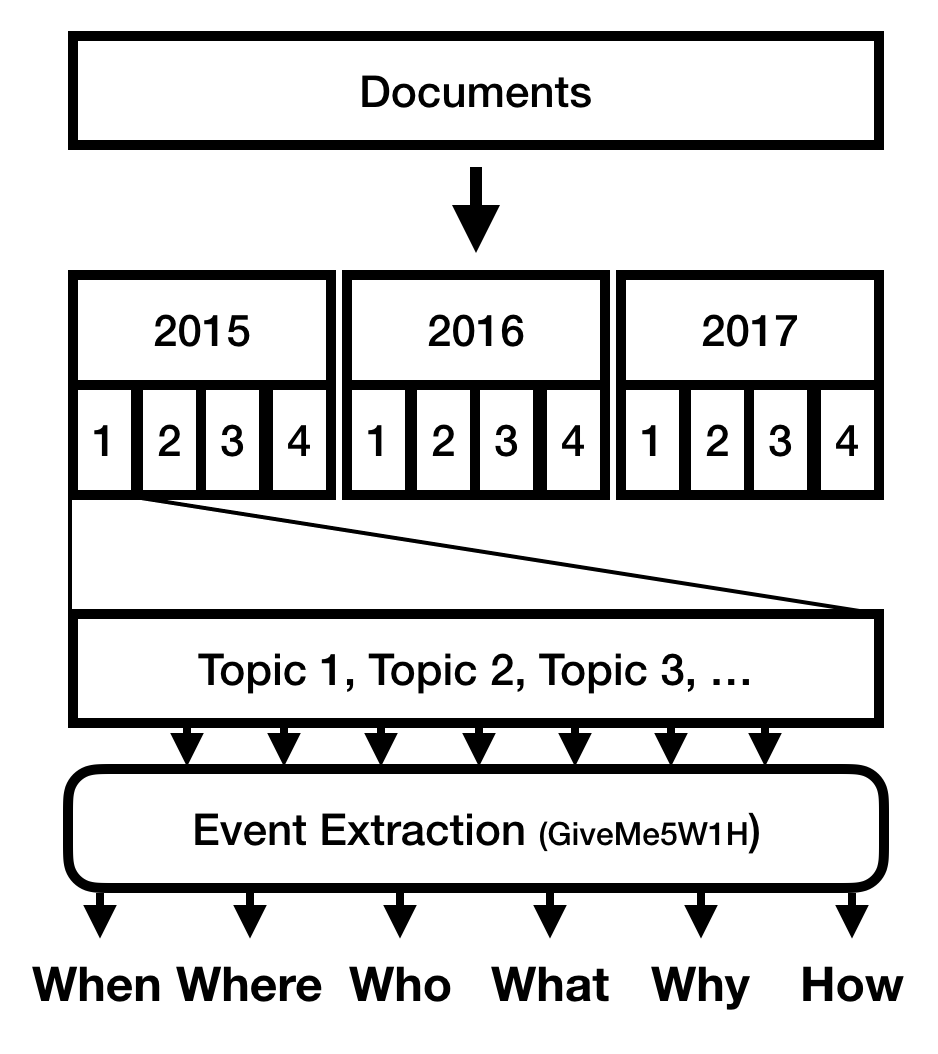
\includegraphics[width=0.8\linewidth]{on_issue_1.png}
  \caption{A brief diagram of on-issue tracking process.}
  \label{fig:onissuedia}
\end{figure}

\subsection{Monthly Division}

We divided all news articles monthly.
The groups contain news articles those are written in \textit{January 2015, Febuary 2015, \dots, December 2017, January 2018}.
\textit{2018 Jan.} group contains only a few articles,
so we decided to ignore the last group.
The reason why we divided the data monthly is, the month is one of the standard in the field of yearly statistics analysis.
For example, the issue about MERS started from May 2015, and ended in January 2016.
If we divide yearly, there will be only one or two groups for extracting events.
Else if we divide quarterly, there will be three or four events.
We can extract eight or nine events from the period if we divide the events mothly,
so this is just fit to make a reasonable result.

\subsection{Articles in the Months Categorization}

With LDA model we have trained at trend analysis project,
we classify the documents in the month groups.
If we give a tokenized sentence to the LDA model,
the model outputs the probability for each group.
We choose the group with maximum value, and assign the document to the group.
So, for each month, there are 21 classified groups of news articles.

\subsection{Event Extraction}

For each group we divided from above,
we extract the events with the approach of word frequency.
For this step, we use a Python library called ``giveme5W1H''\cite{Hamborg2019b}.
The library is the state-of-the-art tool for extracting
\textit{when/where/who/what/why/how} features from the document.
The library uses Stanford's CoreNLP library as its basic structure,
and give analysis results when we give a
title, lead, text, and a published date.
We decided to use columns \textit{title}, \textit{description}, \textit{body}, and a \textit{time}
from the given dataset as an input to get a result.
For each group, we count the frequencies of each feature of the articles,
and select the most frequent terms for each feature, treat them as a score.
Then we extract a most relevant article from the monthly group;
For example, if the term `president' occurs twelve times and
`government' occurs six times as \textit{Who} feature,
the news article contains the term `president' as \textit{Who}
takes double scores than the the article about `government'.
The maximum score article's headline is assumed that it is
representing the main event of the month.

We choose two yearly issues from the list, and do event extraction for each issue.
For each month result, we identify an event based on the result and align them on the timeline.

Table \ref{table:onissue} is an example of on-issue tracking of the issue MERS.

\begin{table}[!htbp]
  \begin{tabular}{l|l}
  Month   & Event(headline)                                        \\ \hline
  2015.06 & S. Korea confirms 3 more MERS cases, total rises to 18 \\
  2015.07 & S. Korea reports no new MERS cases for 17th day        \\
  2015.08 & Park gives appointment letter to new health minister   \\
  2015.09 & Moon stakes leadership on party reform                 \\
  2015.10 & 61 isolated after last MERS patient rediagnosed       
  \end{tabular}
  \caption{The example of on-issue tracking of the issue MERS.}
  \label{table:onissue}
\end{table}